\documentclass[11pt, fleqn]{beamer}\usepackage[]{graphicx}\usepackage[]{color}
% maxwidth is the original width if it is less than linewidth
% otherwise use linewidth (to make sure the graphics do not exceed the margin)
\makeatletter
\def\maxwidth{ %
  \ifdim\Gin@nat@width>\linewidth
    \linewidth
  \else
    \Gin@nat@width
  \fi
}
\makeatother

\definecolor{fgcolor}{rgb}{0.345, 0.345, 0.345}
\newcommand{\hlnum}[1]{\textcolor[rgb]{0.686,0.059,0.569}{#1}}%
\newcommand{\hlstr}[1]{\textcolor[rgb]{0.192,0.494,0.8}{#1}}%
\newcommand{\hlcom}[1]{\textcolor[rgb]{0.678,0.584,0.686}{\textit{#1}}}%
\newcommand{\hlopt}[1]{\textcolor[rgb]{0,0,0}{#1}}%
\newcommand{\hlstd}[1]{\textcolor[rgb]{0.345,0.345,0.345}{#1}}%
\newcommand{\hlkwa}[1]{\textcolor[rgb]{0.161,0.373,0.58}{\textbf{#1}}}%
\newcommand{\hlkwb}[1]{\textcolor[rgb]{0.69,0.353,0.396}{#1}}%
\newcommand{\hlkwc}[1]{\textcolor[rgb]{0.333,0.667,0.333}{#1}}%
\newcommand{\hlkwd}[1]{\textcolor[rgb]{0.737,0.353,0.396}{\textbf{#1}}}%
\let\hlipl\hlkwb

\usepackage{framed}
\makeatletter
\newenvironment{kframe}{%
 \def\at@end@of@kframe{}%
 \ifinner\ifhmode%
  \def\at@end@of@kframe{\end{minipage}}%
  \begin{minipage}{\columnwidth}%
 \fi\fi%
 \def\FrameCommand##1{\hskip\@totalleftmargin \hskip-\fboxsep
 \colorbox{shadecolor}{##1}\hskip-\fboxsep
     % There is no \\@totalrightmargin, so:
     \hskip-\linewidth \hskip-\@totalleftmargin \hskip\columnwidth}%
 \MakeFramed {\advance\hsize-\width
   \@totalleftmargin\z@ \linewidth\hsize
   \@setminipage}}%
 {\par\unskip\endMakeFramed%
 \at@end@of@kframe}
\makeatother

\definecolor{shadecolor}{rgb}{.97, .97, .97}
\definecolor{messagecolor}{rgb}{0, 0, 0}
\definecolor{warningcolor}{rgb}{1, 0, 1}
\definecolor{errorcolor}{rgb}{1, 0, 0}
\newenvironment{knitrout}{}{} % an empty environment to be redefined in TeX

\usepackage{alltt}
\usepackage{amsmath}
\usepackage{amssymb}
\usepackage{geometry}
\usepackage{graphicx}
\usepackage{url}
\IfFileExists{upquote.sty}{\usepackage{upquote}}{}
\begin{document}

\begin{frame}
\large
Lecture 11:\\
Inference for Two Means\\
STAT 310, Fall 2020
\normalsize
\end{frame}

%---------------------------------------------
\begin{frame}{Difference Between Two Means}
\begin{itemize}
\item In this lecture we discuss how to construct confidence intervals and perform hypothesis tests for the difference between two populations means $\mu_1 - \mu_2$, where the data come from two independent samples.
\vspace{10pt}
\item Just as with a single sample, we need to check whether certain conditions are satisfied for the confidence interval or hypothesis test to be valid. 
\vspace{10pt}
\item An important question we address is whether the difference between the two population means is significantly different than 0.
\end{itemize}
\end{frame}

%---------------------------------------------
\begin{frame}{Confidence Interval}
Confidence interval for the difference between two population means $\mu_1 - \mu_2$:


$$\bar{x}_1 - \bar{x}_2 \pm t^* \sqrt{\frac{s_1^2}{n_1} + \frac{s_2^2}{n_2}}$$
\vspace{0.75cm}

\begin{itemize}
\item The degrees of freedom for the critical value $t^*$ can be calculated with the formula $df=$ min$(n_1-1, n_2-1)$  
\item The formula for the degrees of freedom computed using software (\texttt{t.test()} function in R) is more complex.\footnote{\url{https://en.wikipedia.org/wiki/Welch\%27s_t-test}}
\end{itemize}
\end{frame}

%---------------------------------------------
\begin{frame}{Hypothesis Test}
Hypothesis test for the difference between two population means:\\
\vspace{5pt}
$H_0: \mu_1 = \mu_2$\\ 
\vspace{5pt}
%the two means are the same
$H_A: \mu_1 \neq \mu_2$\\ 
%the two means are different
\vspace{15pt}

Test Statistic:
\begin{align*}
t = \frac{\bar{x}_1 - \bar{x}_2}{SE} = \frac{\bar{x}_1 - \bar{x}_2}{\sqrt{\frac{s_1^2}{n_1} + \frac{s_2^2}{n_2}}}
\end{align*}

\small
\begin{itemize}
\item The degrees of freedom are the same as the confidence interval.
\item Can also do a one-sided test (e.g., $H_A: \mu_1 > \mu_2$), but we will focus on two-sided tests when comparing two means.
\end{itemize}
\end{frame}

%---------------------------------------------
\begin{frame}{Conditions}
Conditions for a confidence interval or hypothesis test for the difference between two population means:
\vspace{5pt}
\begin{itemize}
\item The data in each group comes from a random sample, or randomized experiment.  Additionally,  the two groups are independent of each other (the cases in the first group are not related to the cases in the second group).
\vspace{5pt}
\item The sample sizes are large ($n_1 \geq 30$ and $n_2 \geq 30$).  Otherwise, if the samples sizes are small, the data in each group should be approximately normal.
\vspace{5pt}
\item There should be no extreme outliers.
\end{itemize}
\end{frame}

%---------------------------------------------
\begin{frame}{Example}
Are action or comedy movies rated higher on IMDb?  Below are some summary statistics for a random sample of 50 action movies and 50 comedy movies rated on IMDb.  Use a hypothesis test to determine whether there is a statistically significant difference between the two means.\\
\vspace{1cm}

\noindent\begin{minipage}[c]{0.38\textwidth}
\begin{center}
\begin{tabular}{l c c }
\hline
        & \multicolumn{2}{c}{IMDb Rating} \\
\hline
        & Action     & Comedy         \\
Mean    & 5.46       & 6.18     \\
SD      & 1.55       & 1.24       \\
n       & 50         & 50 \\
\hline
& \\
& \\
\end{tabular}
\end{center}
\end{minipage}
\begin{minipage}[c]{0.6\textwidth}
\begin{center}
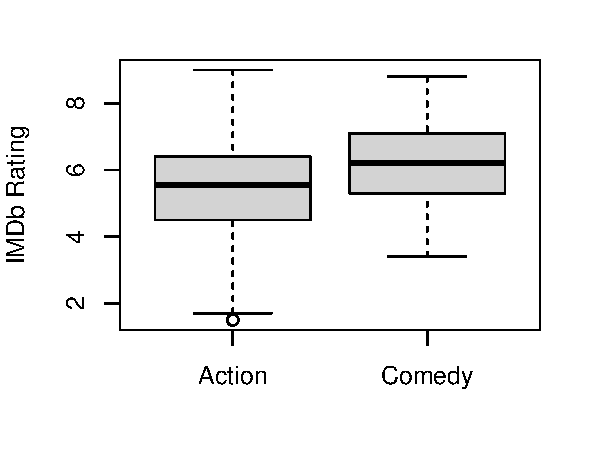
\includegraphics[width=0.75\textwidth]{movie_boxplot.pdf}
\end{center}
\end{minipage}
\end{frame}

\begin{frame}
\small
\begin{enumerate}[(a)]
\item Write the null and alternative hypotheses.
\vspace{0.75cm}
\item Check the conditions for the test.
\vspace{2cm}
\item Calculate the test statistic.
\vspace{2cm}
\end{enumerate}
\end{frame}

\begin{frame}
\small
\begin{enumerate}[(a)]
\setcounter{enumi}{3}
\item Calculate the $p$-value, and and make a decision using $\alpha = 0.05$ significance level.\\
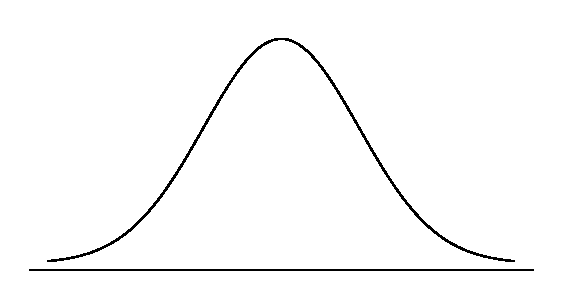
\includegraphics[scale=0.4]{norm_draw.pdf}
\vspace{1cm}

\item What is the conclusion of the test in the context of the data?
\vspace{3cm}
\end{enumerate}
\end{frame}

%---------------------------------------------
\begin{frame}{Example}
Calculate and interpret a 95\% confidence interval for the difference between the mean rating of action and comedy movies on IMDb.
\vspace{7cm}
\end{frame}


\end{document}
